\chapter{Язык механизмов}
Как выглядит аукцион, если не вдаваться в детали? Природа случайно раздает игрокам сигналы. Затем игроки делают ставки. Затем правила аукциона определяют, кто получает товар и кто сколько платит.

Если не обращать внимание на слово «аукцион», то так выглядят абсолютно все задачи, где нужно принять решение. И в этой лекции мы покажем, как аукцион второй цены неплохо справляется со всеми этими задачами!





\section{Описание всех задач на языке механизмов}

Рассмотрим несколько примеров. Во всех примерах нужно выбрать одно решение из нескольких возможных и определить, кто сколько платит. В табличках будут находится полезности игроков в зависимости от принятого решение. Вопрос оплаты решения мы в табличках освещать не будем. Мы также забудем пока про то, что Природа сообщает игрокам какие-то сигналы.\index{язык теории механизмов}


\begin{myex} Аукцион. Есть три игрока и один товар. Ценность товара для них равна $ V_{1} $, $ V_{2} $ и $ V_{3} $. В зависимости от принятого решения, полезности игроков имеют вид:

\begin{tabular}{c|p{2.2 cm}p{2.2 cm}p{2.2 cm}p{2.2 cm}}
& Отдать товар игроку 1 & Отдать товар игроку 2 & Отдать товар игроку 3 & Оставить товар у продавца \\
\hline
Игрок 1 & $ V_{1} $ & 0 & 0 & 0\\
Игрок 2 & 0 & $ V_{2} $ & 0 & 0\\
Игрок 3 & 0 & 0 & $ V_{3} $ & 0\\
\end{tabular}

Можно рассмотреть различные вариации этой задачи. Например, добавить продавца как игрока или убрать решение «Оставить товар у продавца» из списка возможных.

\end{myex}


\begin{myex} \label{bridge}\index{задача!о постройке моста}
Общественное благо. Есть два города, $ A $ и $ B $, на разных берегах реки. Полезность моста для их жителей равна $ V_{A} $ и $ V_{B} $. Есть ещё администрация области, для которой мост обойдется в сумму $ c $.


\begin{tabular}{c|cc}
& Построить мост & Не строить мост \\
\hline
Жители города A & $ V_{A} $ & 0 \\
Жители города B & $ V_{B} $ & 0 \\
Администрация & $-c$ & 0 \\
\end{tabular}

Если администрация тратит не свои деньги, а скажем деньги из какого-то бюджета, который ни на что кроме моста потратить нельзя, тогда её как игрока можно не учитывать, так как ей все равно, строить мост или не строить.

\end{myex}

\begin{myex} \label{pizza} Разносчик пиццы.\index{задача!разносчика пиццы} Есть два клиента, A и B. От ресторана до A ехать $ a $ минут, до B — $ b $ минут. От A до B ехать $ c $ минут. Разносчик может сначала посетить клиента A и затем клиента B, а может и наоборот. Удовольствие клиента от пиццы равно времени доставки со знаком минус.


\begin{tabular}{c|cc}
& сначала к А, потом к B & сначала к B, потом к A \\
\hline
Клиент А & $-a$ & $-b-c$ \\
Клиент B & $-a-c$ & $-b$ \\
\end{tabular}

При желании можно учесть и полезность разносчика пиццы. Например, как общее время доставки со знаком минус. Это будет другая игра. Наш случай означает, что разносчику все равно сколько тратить на дорогу. Скажем, его в ресторане все равно нагрузили бы какой-нибудь работой, если бы он приехал раньше. Можно ещё добавить решения «Ехать только к А», «Ехать только к В» и «Не ехать ни к кому». Но мы будем считать, что пицца безумно вкусна эти варианты даже не рассматриваются клиентами.

\end{myex}


\begin{myex} \label{sm_posuda}\index{задача!о мытье посуды} Мама сказала Саше и Маше помыть посуду и подмести пол. Допустим, что неудовольствие от мытья посуды для каждого из них равно $ (-a) $, а от подметания пола — $ (-b) $.

\begin{tabular}{c|p{2.2 cm}p{2.2 cm}p{2.2 cm}p{2.2 cm}}
& Саша моет посуду, Маша — пол. & Саша моет пол, Маша — посуду. & Всё моет Саша. & Всё моет Маша. \\
\hline
Саша & $ -a $ & $ -b $ & $ -a-b $ & $ 0 $ \\
Маша & $ -b $ & $ -a $ & $ 0 $ & $ -a-b $ \\
\end{tabular}

\end{myex}


Итак, любой механизм решения задачи должен состоять из двух правил: правило, которое говорит, какое решение должно быть принято, и правило, которое говорит, кто и сколько платит.

Некая дополнительная сложность состоит в том, что в реальности часто применяются случайные механизмы решения этих задач. В частности, Саша и Маша могут просто подкинуть монетку, чтобы принять решение. Поэтому правило выбора будет говорить, какими должны быть вероятности принятия каждого из решений.

Итого, для описания механизмов нам понадобятся множества:

\begin{enumerate}
\item $ T_{i} $ — множество всех возможных сигналов\index{множество!возможных сигналов}, которые Природа может послать игроку $ i $. В наших трёх предыдущих лекциях — множество возможных значений случайной величины $ X_{i} $. ещё говорят, множество возможных типов игрока $ i $.

Пример. Пусть каждый игрок знает своё $ X_{i} $. Величины $ X_{i}  $ равномерны на $ [0;1] $. В этом случае $ T_{i}=[0;1] $. Число $ x_{1} $, конкретный сигнал, который получил первый игрок — это элемент из $ T_{1} $.
\item $ B_{i} $ — множество\footnote{Не путайте с другими обозначениями! $ b_{i} $ — это конкретная ставка игрока $ i $, число; $ Bid_{i} $ — ставка игрока как случайная величина; $ b(x) $ — функция, которая говорит, какую ставку делать в зависимости от сигнала.}  всех возможных ходов игрока $ i $.

Например, для аукциона первой цены — это список возможных ставок игрока $ i $, $ B_{i}=[0;+\infty) $. Число $ b_{1} $, конкретная ставка, которую сделал первый игрок — это элемент из $ B_{1} $.

\item $ B=B_{1}\times B_{2}\times \ldots B_{n} $ — декартово произведение множеств ходов отдельных игроков. Множество $B$ — это набор всех возможных сочетаний ходов для наших игроков.\index{множество!возможных ходов}

\item $ T=T_{1}\times T_{2}\times \ldots T_{n} $ — декартово произведение множеств типов отдельных игроков. Множество $T$ — это набор всех возможных сочетаний типов для наших игроков.\index{множество!возможных типов игрока}

\item $ \Delta $ — множество вероятностных распределений на списке решений.\index{множество!вероятностных распределений}

Звучит страшно, но достаточно привести в пример пару элементов из $ \Delta $, чтобы всё стало понятнее. Если мы выбираем между решениями $ a $, $ b $ и $ c $, то элементами $ \Delta $, например, будут: $ \{ $Принять решение $ a\} $, $ \{ $Принять решение $ b $ с вероятностью 0.1 и решение $c$ с вероятностью 0.9 $ \}$.

С математической точки зрения, если у нас $ k $ возможных решений, то $ \Delta $ — это все возможные векторы вероятностей:
\begin{equation}
\Delta=\left\{(p_{1},p_{2},\ldots,p_{k})|\forall p_{i}\geq 0, \sum p_{i}=1 \right\}
\end{equation}

Можно считать, что $ \Delta $ — это множество случаных величин значением которых является одно из решений.
У нас, правда, $ \Delta $ уже использовалась для обозначения маленького числа. Но из контекста всегда понятно, подразумевается ли под $ \Delta $ число или множество вероятностных распределений.

\end{enumerate}

В этих обозначениях, например, стратегия $ i $-го игрока — это функция $ s_{i}:T_{i}\to B_{i} $. Кстати, равновесие Нэша — это набор стратегий по одной от каждого игрока, то есть это функция $ NE:T\to B $. Действительно, если заданы типы всех игроков и задано равновесие Нэша, то мы можем понять, какие ходы будут сделаны. Естественно, равновесие Нэша, это не произвольная такая функция — нужно ещё сказать, что никому не будет выгодно отклоняться, если все игроки расскажут друг другу свои стратегии.

А механизм — это правила игры:

\begin{mydef} \indef{Механизм}\index{механизм}. Описание механизма состоит из трёх пунктов:
\begin{enumerate}
\item $ B_{i} $ — список возможных ходов игрока $ i $.
\item $Q:B\to \Delta  $ — правило распределения: функция, которая определяет вероятности принятия каждого решения в зависимости от ходов игроков.
\item $M:B\to \mathbb{R}^{n}  $ — правило платежей: функция, которая определяет кто и сколько платит в зависимости от ходов игроков.
\end{enumerate}
\end{mydef}

Вообще говоря список ходов $ B_{i} $, предлагаемый игроку $ i $ может быть произвольным и никак не связанным со списком $ T_{i} $ возможных состояний игрока $ i $.

\begin{myex}
Три игрока и один товар. Для игрока $ i $ товар имеет ценность $ X_{i} $, каждый игрок знает своё $ X_{i} $. Величины $ X_{i}  $ независимы и равномерны на $ [0;1] $.

В этом примере $ T_{i}=[0;1] $. Но это никак не ограничивает нас в множестве ходов. Например, мы можем попросить наших трёх игроков одновременно в разных комнатах станцевать вальс. В этом случае $B_{i} =\{ $Множество возможных вальсов$\}$.
\end{myex}

Подобные механизмы использует Дед Мороз в детском саду: «Кто расскажет самый лучший стишок\ldots» и тамада на свадьбе «Кто назовёт больше всего комплиментов невесте\ldots».

Мы же ограничимся прямыми механизмами\index{механизм!прямой}. Прямой механизм прямо спрашивает у каждого игрока: «Ты кто?». Точнее говоря, «Ты какого типа?» или «Какой сигнал послала тебе природа?». Игрок при этом может сказать правду, а может и соврать. В прямом механизме множество возможных ходов совпадает с множеством типов игрока, $ T_{i}=B_{i} $

\begin{mydef} \indef{Прямой механизм}. В прямом механизме $ B_{i}=T_{i} $ и его описание включает в себя:
\begin{enumerate}
\item $ Q:B\to \Delta $ — правило распределения: функция, которая определяет вероятности принятия каждого решения в зависимости от объявленных игроками своих типов.\index{правило распределения}
\item $ M:B\to \mathbb{R}^{n}  $ — правило платежей: функция, которая определяет, кто и сколько платит в зависимости от объявленных игроками своих типов.\index{правило платежей}
\end{enumerate}
\end{mydef}


Рассмотрим подробнее простую ситуацию. Три игрока и один товар. Для игрока $ i $ товар имеет ценность $ X_{i} $, каждый игрок знает своё $ X_{i} $. Величины $ X_{i}  $ независимы и равномерны на $ [0;1] $. В этом случае: $ T_{i}=[0;1] $.

В рамках этой ситуации рассмотрим наши три аукциона на языке механизмов.

%Чтобы разом решить проблему совпадения ставок нам потребуется ещё одно несложное обозначение. Пусть игроки сделали ставки $ \vec{b} $.
%\begin{mydef}
%Обозначим $ players(\vec{b},k) $ — вектор из нулей и единиц, где единицы стоят для тех игроков, которые сделали $ k $-ые по величине ставки. Обозначим также $ \#players(\vec{b},k) $ — количество игроков, сделавших $ k $-ую по величине ставку. Саму $ k $-ую по величине ставку обозначим буквой $ M_{k}(\vec{b}) $.
%\end{mydef}

%\begin{myex} Если $ \vec{b}=(2,3,4,5,2,5) $, то  $ players(\vec{b},1)=(0,0,0,1,0,1) $, $ players(\vec{b},2)=(0,0,1,0,0,0) $, $ \#players(\vec{b},1)=2 $, $\#players(\vec{b},2)=1$. Кроме того, $ M_{1}(\vec{b})=5 $, $ M_{2}(\vec{b})=4 $.
%\end{myex}

%Можно, например, связать с помощью скалярного произведения:
%\begin{equation}
%M_{1}=\frac{\vec{b}\cdot players(\vec{b},1) }{\#players(\vec{b},1)}
%\end{equation}

%Или:
%\begin{equation}
%\#players(\vec{b},k)=players(\vec{b},k)\cdot players(\vec{b},k)
%\end{equation}


\begin{myex} Аукцион первой цены. Товар достаётся тому, кто назвал наибольшую цену. Если таких игроков несколько — выбираем победителя из них наугад. Победитель платит названную им самим цену.\index{аукцион!первой цены}

Можно считать, что механизм прямой и множество разрешенных ходов имеет вид $B_{i}=T_{i}=[0;1] $.

Функция $ Q(\vec{b}) $ говорит нам, с какой вероятностью побеждает тот или иной игрок при заданном $ \vec{b} $.

Например, пятый игрок назвал цену выше всех:
\begin{equation}
Q(1,2,3,4,5)=(0,0,0,0,1)
\end{equation}

Или, второй и третий игрок назвали наибольшую цену:
\begin{equation}
Q(1,3,3,1,2)=(0,0.5,0.5,0,0)
\end{equation}

То есть функция $ Q $ расставляет равные вероятности для игроков с наибольшей ставкой.

А соответственно функция $ M(\vec{b}) $ говорит, что только победитель платит. Но победитель выбирается наугад среди игроков с наибольшей ставкой, поэтому у всех игроков с наибольшей ставкой есть ожидаемый платеж.

Например, если пятый игрок назвал цену выше всех:
\begin{equation}
M(1,2,3,4,5)=(0,0,0,0,5)
\end{equation}

Или, второй и третий игрок назвали наибольшую цену:
\begin{equation}
M(1,3,3,1,2)=(0,1.5,1.5,0,0)
\end{equation}




%Функция распределения задает вероятности получения товара каждым игроком:
%\begin{equation}
%\winpro(\vec{b})=\frac{1}{\#players(\vec{b},1)}\cdot players(\vec{b},1)
%\end{equation}

%Функция $ \mu(\vec{b}) $ должна описывать какой средний платеж должны сделать игроки, если известны их ставки. В нашем случае %платит только победитель. Но победитель выбирается наугад среди игроков с наибольшей ставкой, поэтому у всех игроков с наибольшей ставкой есть ожидаемый платеж:
%\begin{equation}
%\mu(\vec{b})=\frac{M_{1}(\vec{b})}{\#players(\vec{b},1)}\cdot players(\vec{b},1)
%\end{equation}

\end{myex}

\begin{myex} Аукцион второй цены. Товар достаётся тому, кто назвал наибольшую цену. Если таких игроков несколько — выбираем победителя из них наугад. Победитель платит вторую по величине цену.\index{аукцион!второй цены}

Можно считать, что механизм прямой и множество разрешенных ходов имеет вид $B_{i}=T_{i}=[0;1] $.

Функция $ Q(\vec{b}) $ точно такая же, как на аукционе первой цены, так как победитель — это тот, кто назвал наибольшую ставку.

Функция $ M(\vec{b}) $ отличается. Она говорит, что победитель платит не свою, а вторую по величине ставку.

Например,
\begin{equation}
M(1,2,3,4,5)=(0,0,0,0,4)
\end{equation}

Или,
\begin{equation}
M(1,3,3,1,2)=(0,1,1,0,0)
\end{equation}
Единица — взялась от деления двойки (второй по величине цены) на двух потенциальных победителей.

\end{myex}

\begin{myex} Кнопочный аукцион.\index{аукцион!кнопочный}

Кнопочный аукцион не является прямым механизмом, так как множество возможных ходов существенно сложнее множества сигналов, которые может получить игрок. Полное описание этого аукциона с выписыванием функций $ Q $ и $ M $ в явном виде  занудно. Поэтому мы ограничимся описанием множеств $ B_{i} $. Зная выбор каждого игрока из его множества $ B_{i}$, мы можем определить, кто выиграл и сколько ему нужно платить, значит, функции $ Q $ и $ M $ существуют.

Представим себе, что первый игрок знает значение  своего сигнала $ X_{1} $. Ему нужно решить, до какой цены жать кнопку, пока кнопку жмут трое, то есть нужно выбрать некое число в диапазоне $ [0;1] $. ещё нужно решить до какой цены жать кнопку, когда осталось двое игроков, а самый слабый вышел на цене $ p $, то есть нужно выбрать некую непрерывную на $ [0;1] $ функцию.

В результате $ B_{i}=[0;1]\times C[0;1] $, то есть $ B_{i} $ — это декартово произведение отрезка $ [0;1] $ на множество непрерывных на отрезке $ [0;1] $ функций.

Для примера найдём $ Q(\vec{b})$ и $ M(\vec{b}) $ в точке  $\vec{b}=((0.7,p+p^{2}),(0.5,2p),(0.8,p+p^{3})) $. В данных условиях первым выйдет второй игрок, так как он жмет кнопку до момента времени $ t=0.5 $. Далее останутся первый и третий игрок, которые подставят в свои функции $ p=0.5 $. Значит, первый будет жать кнопку до $ t=0.75 $, а третий — до $ t=0.625 $. Аукцион окончится в $ t=0.625 $ победой первого игрока:
\begin{equation}
Q((0.7,p+p^{2}),(0.5,2p),(0.8,p+p^{3}))=(1,0,0)
\end{equation}
И
\begin{equation}
M((0.7,p+p^{2}),(0.5,2p),(0.8,p+p^{3}))=(0.625,0,0)
\end{equation}

Лишний раз стоит подчеркнуть, что $ (0.7,p+p^{2}) $ — это ход первого игрока. А стратегия игрока — это функция, которая говорит, какой элемент из $ B_{i} $ выбирать в зависимости от полученного сигнала из $ T_{i} $. Стратегия это правило, которое каждому числу из $ T_{i}=[0;1] $ сопоставляет конкретный ход, то есть пару (число, функция) из $ B_{i} $

\end{myex}

Мы считаем, что организаторы честно исполняют описанные в механизме функции, даже если после того, как они узнали ставки, им стало выгодно изменить механизм. Это, конечно, не всегда так, и тут уместно сделать небольшое лирическое отступление.

В поезде Москва-Амстердам перегонщиком машин из Белоруссии была рассказана следующая история\index{история перегонщика машин}. Он купил машину на аукционе за 1200 евро, перегнал, дал объявление о продаже за 2000. Звонков много, и всем он сказал, что она уже продана. Потом дал новое  объявление о продаже за 2500. Звонков много, и всем он снова сказал, что она уже продана. И так далее. Продал он её, то ли за 3500, то ли за 3800, не помню.

Именно поэтому в реальности на многих аукционах есть стартовая цена, а есть резервная цена и это не одно и тоже. Стартовая цена — это цена с которой начинаются торги. Естественно, товар не может быть продан ниже стартовой цены. Стартовую цену игроки знают, а резервная цена известна только организаторам аукциона. Если торги не доходят до резервной цены, то товар остаётся у продавца, но он получает информацию о ставках. А если бы продавец начал торг с резервной цены, то он бы не получил информацию о ставках, так как их бы не было.


\section{Правдивость и другие желательные свойства}

Когда механизм принятия решения объявлен игрокам, игроки будут выбирать свои стратегии. Какой механизм выбрать, чтобы в равновесии Нэша были достигнуты определенные цели?

А теперь чудо-замена превращается в чудо-теорему, объясняющую почему можно изучать только прямые механизмы. Оказывается, любой механизм можно изменить так, чтобы он стал прямым, а игрокам было бы выгодно правдиво декларировать свои типы. При этом ни принимаемое решение, ни платежи никак не изменятся!

\begin{myth} \label{revelation_principle}\index{теорема!о существовании прямого механизма}
Пусть задан произвольный механизм $ (B, Q, M) $ и равновесие Нэша $NE$ в нем. Существует прямой механизм $ (Q', M') $ и равновесие Нэша $NE'$ в нем такое, что:
\begin{enumerate}
\item При любых типах игроков вероятностям принятия решений и платежи в равновесиях $ NE $ и $ NE' $ совпадают.
\item В равновесии $ NE' $ игроки правдиво сообщают свои типы.
\end{enumerate}
\end{myth}

\begin{proof}
Давайте вспомним логику нашей чудо-замены\index{чудо-замена}. Для конкретности можно представлять себе аукцион первой цены с симметричными игроками, но это нигде в доказательстве не используется.

Первый игрок, зная $ x $, максимизирует функцию $ \pi_{1}(x,b_{1}) $ по $ b_{1} $. При этом получается некое оптимальное $ b_{1}^{*} $.

Мы говорили: давайте заменим $ b_{1}=b(a) $. И будем максимизировать по $ a $. Неважно, что функция $ b() $ пока ещё неизвестна. Важно, нам заранее известен результат оптимизации по $ a $. С одной стороны, должно быть $ b_{1}^{*}=b(a^{*})$, а с другой стороны, функция $ b() $ — это равновесная стратегия, поэтому $ b_{1}^{*}=b(x) $. И при хороших свойствах $ b() $ из этого следует, что  $ a^{*}=x $.

Что будет если мы реализуем нашу чудо-замену в реальности? То есть продавец обещает игрокам: «Вы мне говорите $ a $, а я за вас сделаю ставку $ b(a) $ на аукционе». Что тогда оптимально говорить игрокам? Игрокам оптимально говорить $ a^{*}=x $, то есть правдиво сообщать ценность товара для себя.

Если организаторы аукциона будут сначала применять функцию $ b() $ к ходам игроков, а затем использовать старый механизм, то игрокам будет выгодно правдиво декларировать свои типы.

% #TODO картинка пост-обработки ставки


Если игроки несимметричны, то при старом механизме у каждого игрока своя оптимальная стратегия и равновесие Нэша имело вид $ (b_{1}(x),b_{2}(x),\ldots,b_{n}(x)) $. В этом случае в новом прямом механизме ход первого игрока предварительно обрабатывается функцией $ b_{1}() $, ход второго — функцией $ b_{2}() $ и так далее.

Более формально: Пусть равновесие $ NE $ имеет вид $ \beta: T\to B $. Смысл написанного: равновесие — это функция, которая каждому набору типов игроков ставит в соответствие набор сделанных ими ходов. Если расписывать детально, то
\[
\beta(x_{1},x_{2},\ldots,x_{n})=(b_{1}(x_{1}),b_{2}(x_{2}),\ldots,b_{n}(x_{n})).
\]

Пусть $ \vec{x} $ — произвольный набор типов игроков, $ \vec{x}\in T $. Определим прямой механизм по принципу: $ Q'(\vec{x}):=Q(\beta(\vec{x})) $ и
$ M'(\vec{x}):=M(\beta(\vec{x}))  $.

При этом автоматически оказывается, что при новом механизме равновесие Нэша $ NE' $ будет иметь вид: $ \beta'(x_{1},x_{2},\ldots,x_{n})=(x_{1},x_{2},\ldots,x_{n}) $. Действительно, если бы какому-то игроку  не было выгодно правдиво декларировать свой тип $ x_{i} $ в этой ситуации, то ему не было бы выгодно использовать стратегию $ b_{i}(x_{i}) $ в исходном непрямом механизме.

А если все игроки правдиво декларируют свои ценности, то и результат применения прямого механизма совпадает с результатом применения исходного непрямого механизма.
\end{proof}

Применим нашу теорему к аукциону первой цены.\index{аукцион!первой цены}

\begin{myex} Когда мы решали аукцион первой цены в простейшем случае, $ X_{i}=V_{i} $, ценности $ X_{i} $ независимы и равномерны на $ [0;1] $ мы установили, что оптимальная стратегия имеет вид $ b(x)=\frac{n-1}{n} x$.

Теорема говорит нам, что можно так поменять правила аукциона, что никому ни хуже ни лучше не станет, но игроки будут говорить правду. Как это сделать?

Изменим правила аукциона. Победителем по прежнему будем считать игрока с наибольшей ставкой. А вот платить он будет не ровно свою ставку, а свою ставку, умноженную на $ \frac{n-1}{n} $. Каждый игрок знает, что его ставка будет автоматом помножена на $ \frac{n-1}{n} $. Значит, теперь каждому выгодно говорить правду. А фактические платежи и победитель не поменялись!
\end{myex}

На аукционе второй цены игроки говорят правду и без каких-то поправок.

Теперь вместо того, чтобы изучать произвольные механизмы и произвольные равновесия Нэша в них, можно ограничиться изучением прямых механизмов и равновесий Нэша в которых игроки правдиво заявляют свой тип. То есть можно никогда не делать разницы между множествами $ B_{i} $ и $ T_{i} $. Кроме как на свадьбе и в детском саду :)

Существует несколько свойств, которые мы хотели бы видеть у механизмов:

\begin{mydef}
\indef{Правдивость}\index{механизм!правдивый}. Прямой механизм называется правдивым, если в равновесии Нэша игроки правдиво декларируют свои сигналы.
\end{mydef}

\begin{myex}
Будем считать, что выполнены предпосылки теоремы об одинаковой доходности. Аукцион первой цены не правдив, аукцион второй цены правдив.
\end{myex}

\begin{mydef} \indef{Эффективность}\index{механизм!эффективный}. Механизм называется эффективным, если в равновесии Нэша принятое решение максимизирует суммарную полезность всех агентов.
\end{mydef}

\begin{myex} Если выполнены предпосылки теоремы об одинаковой доходности, то аукционы первой и второй цены является эффективными механизмами. Действительно, в этом случае товар достаётся игроку с максимальной полезностью. Любое другое решение приведет к снижению совокупной полезности.
\end{myex}

Нужно подчеркнуть, что эффективность не учитывает правило платежей! Когда мы говорим об эффективности механизма, мы говорим об эффективности правила распределения.

\begin{mydef}
\indef{Индивидуальная рациональность}\index{механизм!индивидуально рациональный}. Механизм называется индивидуально рациональным, если игроки согласны участвовать в нем добровольно.
\end{mydef}

Индивидуальная рациональность учитывает правило платежей! Когда мы говорим об индивидуальной рациональности, мы учитываем и правило распределения и правило платежей.

\begin{myex} Если выполнены предпосылки теоремы об одинаковой доходности, то аукционы первой и второй цены индивидуально рациональны, так как ожидаемый выигрыш каждого игрока неотрицательный. А пример \ref{sm_posuda} с Сашей и Машей, которым нужно помыть пол и посуду не будет индивидуально рациональным, если только мама не предложит им какую-нибудь компенсацию в виде похода в кино.
\end{myex}

\begin{mydef} \indef{Оптимальность}\index{механизм!оптимальный}. Механизм называется оптимальным, если в равновесии Нэша организаторы получают от игроков максимально возможную ожидаемую прибыль.
\end{mydef}

Если у нас есть диктаторские полномочия, то есть мы можем заставить игроков участвовать в аукционе, то, очевидно, мы можем получить сколь угодно большую прибыль. Для этого просто надо потребовать от каждого заплатить достаточно много. Но такой аукцион не будет индивидуально рациональным. Поэтому обычно выбирают оптимальный механизм среди индивидуально рациональных.

Иногда организаторам не нужно заработать денег. Бывает задача состоит в том, чтобы организовать игру так, чтобы в равновесии Нэша было принято некое желательное решение. Скажем, в примере со строительством моста организаторы могут быть заинтересованы в принятии решения «построить мост». То есть нам интересно принятие нужного решения, а не потоки платежей, которые возникают в связи с этим. В этом случае от механизма может требоваться:

\begin{mydef} \indef{Бюджетная сбалансированность}\index{бюджетная сбалансированность механизма}. Механизм имеет сбалансированный бюджет, если в равновесии Нэша сумма платежей всех игроков равна нулю.
\end{mydef}

Стоит сразу сказать, что не всех этих свойств можно добиться одновременно. Для некоторых задач доказано, что не существует механизма, который был бы эффективен, правдив, индивидуально рационален и бюджетно сбалансирован.


\section{Механизм VCG}

Есть универсальный механизм, который применим к множеству ситуаций. Этот механизм есть не что иное, как аукцион второй цены. Давайте повнимательнее к нему присмотримся\ldots~Мы сознательно пока забудем про платежи и сосредоточимся только на полезности от получения товара.


%Давайте ответим на очень простой вопрос на аукционе второй цены.

Конкретный пример. У пяти игроков были ценности равные $ (1,3,7,11,25) $. Ровно такие ставки они и сделали. Победил пятый игрок, который поставил 25.  При этом он получил от товара полезность равную 25. Остальные четверо получили суммарную полезность 0.

А что произошло бы если бы пятый не участвовал в аукционе? Тогда победил бы игрок с ценностью 11. При этом четверо игроков (кроме нынешнего пятого) получили бы суммарную полезность, равную 11.

Заметим, что при удалении любого другого игрока сумма полезностей остальных (без учета платежей) не поменялась бы.

Подводим итог. На аукционе второй цены выплата $i$-го игрока равна максимально достижимой суммарной полезности всех игроков, кроме $i$-го, за вычетом текущей суммарной полезности всех игроков, кроме $i$-го.

Механизм Викри-Кларка-Гровса применяет эту идею к любой задаче.

\begin{mydef} \indef{Механизм VCG}. \index{механизм!VCG}Неформальное определение:
\begin{enumerate}
\item Правило распределения: выбрать решение, максимизирующее сумму полезностей.
\item Правило платежей: игрок $ i $ платит суммарную потерю полезности остальных игроков от своего участия в игре.
\end{enumerate}
\end{mydef}

Опишем идею немножко более формально. Пусть множество возможных типов игрока $ i $ — это числовое множество $ T_{i} $, чаще всего отрезок. Мы рассматриваем только прямые механизмы, поэтому множество возможных ходов такое же, $ B_{i}=T_{i}$.

Полезность игрока зависит от его типа и принятого решения, $ v_{i}(X_{i},w) $. то есть типовая табличка имеет вид:

\begin{tabular}{c|cc}
& Решение $ w_{1} $ & Решение $ w_{2} $ \\
\hline
Игрок 1 & $v_{1}(X_{1},w_{1})$ & $v_{1}(X_{1},w_{2})$ \\
Игрок 2 & $v_{2}(X_{2},w_{1})$ & $v_{2}(X_{2},w_{2})$ \\
Игрок 3 & $v_{3}(X_{3},w_{1})$ & $v_{3}(X_{3},w_{2})$ \\
\end{tabular}

%Единственное, что нужно уточнить — это как трактовать игру без игрока $ i $. Подходящая нам трактовка такова — сигнал игрока $ i $ имеет наименьшее возможное значение, то есть $ X_{i}=\alpha_{i} $.

В теореме мы используем обозначения:

\begin{enumerate}
\item $b_{i}$ — ход, сделанный игроком $ i $, поскольку механизм прямой, это есть заявленный им тип.
\item $w^{*}$ — решение максимизирующее суммарную полезность всех игроков при типах $ (b_{1},b_{2},\ldots,b_{n}) $.
\item $w_{-i}^{*} $ — решение максимизирующее суммарную полезность всех игроков кроме игрока $ i $ при типах $ (b_{1},b_{2},\ldots,b_{n}) $. Заметим, что в данном случае неважно, какой тип у $ i $-го игрока, поскольку о его полезности не заботятся.
\end{enumerate}

Итак,
\begin{mydef} \indef{Механизм VCG}\index{механизм!VCG}, механизм Викри-Кларка-Гровса — это прямой механизм, в котором:
\begin{enumerate}
\item Множество $ B_{i}=T_{i} $, то есть каждому игроку предлагают сказать свой тип.
\item Правило распределения: выбирается то решение $ w $, которое максимизирует сумму полезностей игроков при задекларированных ходах. Если таких решений несколько, то оно выбирается равновероятно.
\begin{equation}
\max_{w} \sum_{i} v_{i}(b_{i},w)
\end{equation}
\item Правило платежей: платеж $ i $-го игрока есть разница между: максимально возможной суммарной полезностью остальных игроков, если $ i $-ый не участвует в игре, и суммарной полезностью остальных игроков при текущем решении.
\begin{equation}
M_{i}(\vec{b})=\sum_{j\neq i} v_{j}(b_{j},w_{-i}^{*})-\sum_{j\neq i} v_{j}(b_{j},w^{*})
\end{equation}
\end{enumerate}
\end{mydef}

Мы сейчас докажем, что в механизме VCG стратегия игрока «правдиво декларировать свой тип» нестрого доминирует все остальные. Но перед доказательством разберём пару примеров:

\begin{myex}
Применение механизма VCG к разносчику пиццы, \ref{pizza}.\index{задача!разносчика пиццы}

Сначала определим, какое решение примет механизм VCG. Для этого посчитаем сумму полезностей.

\begin{tabular}{p{3 cm}|p{3 cm}p{3 cm}}
& сначала к А, потом к B & сначала к B, потом к A \\
\hline
Клиент А & $-a$ & $-b-c$ \\
Клиент B & $-a-c$ & $-b$ \\
Сумма полезностей& $-2a-c$ & $-2b-c$ \\
\end{tabular}

То есть механизм VCG выберет наикратчайший путь. Для определенности будем считать, что $ a<b<c $. В этом случае, разносчик пиццы едет сначала к А, потом к В.

Теперь определим для случая $ a<b $, кто и сколько платит.

Сколько платит игрок А? Если бы A не было, то оптимальным был бы путь к В напрямую и тот получил бы полезность $ -b $. Сейчас B получает полезность $ -a-c $. Стало быть игрок А должен заплатить $ -b-(-a-c)=a+c-b $.

Сколько платит игрок В? Если бы B не было, то оптимальным был бы путь к А напрямую и тот получил бы полезность $ -a $. Сейчас А получает полезность $ -a $. Стало быть игрок В ничего не платит, $ -a-(-a)=0 $.
\end{myex}

\begin{myex}
Применение механизма VCG к строительству моста, \ref{bridge}\index{задача!о постройке моста}. Для примера возьмем конкретные значения $ V_{A} $, $ V_{B} $ и $ c $. Посчитаем сумму полезностей. Зная сумму определим, какое решение примет VCG.

\begin{tabular}{c|cc}
& Построить мост & Не строить мост \\
\hline
Жители города A & $ +60 $ & 0 \\
Жители города B & $ +90 $ & 0 \\
Администрация & $-100 $ & 0 \\
Сумма & +50 & 0 \\
\end{tabular}

Механизм VCG говорит, что мы строим мост.

Теперь считаем, кто и сколько платит.

Сколько платят жители А? Если бы их не было, то оптимальным было бы решение не строить мост и остальные игроки получили бы полезность 0. Сейчас остальные игроки получают в сумме $ (-10) $. Значит, жители $ A $ платят $ 0-(-10)=10 $.

Сколько платят жители В? Если бы их не было, то оптимальным было бы решение не строить мост и остальные игроки получили бы полезность 0. Сейчас остальные игроки получают в сумме $ (-40) $. Значит, жители В платят $ 0-(-40)=40 $.

Тут мы видим существенный недостаток механизма VCG, а именно бюджетную несбалансированность. Чтобы сделать то, что советует VCG, нужно взять откуда-то с потолка ещё 50 рублей. И это проблема не конкретно механизма VCG, а именно принципиальная несовместимость некоторых желательных свойств механизмов.
\end{myex}

Естественно возникает вопрос, а как механизм VCG добьется того, чтобы максимизировать суммарную полезность? Ведь для этого надо знать истинные полезности игроков! А вдруг они соврали, когда сообщали свои типы? Ответ, естественно, состоит в том, что игрокам выгодно правдиво сообщать свои типы:

\begin{myth}\index{теорема!о правдивости механизма VCG}
При использовании механизма VCG стратегия «Правдиво декларировать свой тип, $ b_{i}(x_{i})=x_{i} $» нестрого доминирует остальные стратегии игрока $ i $.
\end{myth}


\begin{proof}
Посчитаем полезность первого игрока полезность в случае, если игроки делают ходы $ (b_{1},\ldots,b_{n}) $, необязательно правдивые.

Общая полезность с учётом решения и платежа равна
\begin{multline}
v_{1}(x_{1},w^{*})-M_{1}=v_{1}(x_{1},w^{*})-\left(\sum_{j=2}^{n}v_{j}(b_{j},w_{-1}^{*})-\sum_{j=2}^{n}v_{j}(b_{j},w^{*})\right)=\\
=v_{1}(x_{1},w^{*})+\sum_{j=2}v_{j}(b_{j},w^{*})-\sum_{j=2}^{n}v_{j}(b_{j},w_{-1}^{*})
\end{multline}

Первый игрок выбирает $ b_{1} $. На что оно влияет? Оно влияет только на исход $ w^{*} $! Первый игрок не в силах изменить, ни  $ w_{-1}^{*} $, так как это игра без него, ни ходы $ b_{j} $ остальных игроков. то есть выбор хода $ b_{1} $ не меняет вычитаемого.

Оставшиеся два слагаемых, на которые первый игрок может влиять выбором хода $ b_{1} $, — это не что иное, как суммарная полезность всех игроков, если бы их типы были бы равны $ (x_{1},b_{2},b_{3},\ldots,b_{n}) $.

А правило распределения $ w^{*} $ обеспечивает максимизацию суммарной полезности для задекларированных типов $ (b_{1},b_{2},\ldots,b_{n}) $. Значит, если первый игрок сообщит $ b_{1}=x_{1} $, то правило $ w^{*} $ само максимизирует его полезность.

\end{proof}

Следовательно, профиль стратегий, где все игроки правдиво декларируют свой тип, является равновесием Нэша.


%Есть небольшая вариация этого механизма, механизм AVG.


%Упражнение:
%Опишите механизм AVG для аукциона трёх игроков.



Есть и другой подход к обобщению идеи аукциона второй цены. И этот подход также активно используется.

\begin{myex} Обобщенный аукцион второй цены, Generalized Second Price auction, GSP.\index{аукцион!второй цены обобщённый}

Как Google делает деньги? Около 98\% своих денег Google делает на продаже рекламных ссылок. Есть несколько рекламных мест, которые показываются, когда пользователь запрашивает в поисковике какое-нибудь слово, например «Абрикос». Эти места отличаются по престижности. А именно, места отличаются по среднему количеству переходов в час, «кликов» мышкой по ссылке.

У каждого игрока есть мнение о ценности одного «клика». Желающие получить эти рекламные места одновременно делают свои ставки.

Игрок, сделавший самую большую ставку, получает самое престижное место, игрок, сделавший вторую по величине ставку, получает второе по престижности место и так далее.  При этом победитель платит за каждый «клик» не свою ставку, а вторую по величине ставку; игрок получивший второе по престижности место платит за каждый «клик» ставку игрока, получившего третье по престижности место и так далее. Игрок выигравший самое непрестижное рекламное место, платит за каждый «клик» самую высокую ставку среди игроков, которые ничего не выиграли.

Есть ещё разные тонкости, но основная идея верна. Желающие могут сами поиграться на \url{adwords.google.com}. Например, за сумму в несколько долларов можно сделать страницу-сюрприз, которая будет выводиться первой при поиске на фразу «день рождения Васи Петрова».
\end{myex}


% Но все же общим корнем VCG и GSP является аукцион второй цены.



\section{Оптимальный аукцион}

А сейчас мы увидим, что в простейшей ситуации аукцион второй цены с резервной ценой оптимален.

Пусть каждый покупатель знает ценность товара для себя, то есть  $ X_{i}=V_{i} $. Кроме того предположим, что каждая ценность имеет регулярное распределение, описываемое функцией распределения $ F_{i}(x) $.

Что произошло бы, если бы никакого аукциона не было, и продавец просто предложил бы каждому покупателю купить у него товар по цене $ x $? В этом случае игрок $ i $ согласился бы на покупку, если $ X_{i}>x $, а вероятность этого равна:
\begin{equation}
\P(X_{i}>x)=1-F_{i}(x)
\end{equation}

И при отсутствии аукциона, средний доход продавца от $ i $-го игрока был бы равен:
\begin{equation}
TR_{i}=x(1-F_{i}(x))
\end{equation}

По сравнению с обычной формулой $ TR(Q)=\P(Q)\cdot Q $:
\begin{enumerate}
\item $ x $ — это аналог цены $ \P(Q) $
\item $ 1-F_{i}(x) $ — это аналог количества товара $ Q $
\end{enumerate}

Как обычно в экономике можно определить предельный доход продавца, $ TR'(Q) $:
\begin{multline}
MR_{i}(x)=\frac{d TR_{i}(x)}{d(1-F_{i}(x))}=x+(1-F_{i}(x))\frac{dx}{d(1-F_{i}(x))}=\\
=x+(1-F_{i}(x))\frac{-1}{f(x)}=x-\frac{1-F_{i}(x)}{f_{i}(x)}
\end{multline}
Мы воспользовались тем, что производная обратной функции — это единица делить на производную исходной.
В результате у нас появилось:
\begin{mydef}
\indef{Предельный доход продавца}\index{предельный доход продавца} — это
\begin{equation}
MR_{i}(x)=x-\frac{1-F_{i}(x)}{f_{i}(x)}
\end{equation}
\end{mydef}

Эта величина — скорость роста ожидаемого дохода продавца при росте вероятности сделки. Если она положительна, значит, продавец заинтересован в росте вероятности сделки, то есть в снижении $ v $. Если она отрицательна, значит, продавец заинтересован в снижении вероятности сделки, то есть в росте $ v $.

Оказывается, что величина $ MR_{i} $ возникает и при моделировании аукционов. А именно,

\begin{myth}
\begin{equation}
\E(pay_{1}(X_{1}))=\E(q_{1}(X_{1})MR_{1}(X_{1}))
\end{equation}
\end{myth}

\begin{proof}
Мы будем изучать первого игрока, и поэтому опустим индекс $ 1 $, чтобы было меньше писанины.

Для доказательства вспомним формулу из теоремы об одинаковой доходности первой лекции:
\begin{equation}
pay(x)=xq(x)-\int_{0}^{x}q(t)dt
\end{equation}

Тогда мы считали, что все игроки используют равновесные стратегии. И при этом трактовали функции как:

\begin{itemize}
\item $ q(x) $ — вероятность того, что первый игрок выиграет, если его ценность равна $ x $.
\item $ pay(x) $ — средняя выплата от первого игрока продавцу, если его ценность равна $ x $
\end{itemize}

Теперь представим себе, что как в теореме \ref{revelation_principle}\index{теорема!о существовании правдивого механизма} мы заменили исходный механизм прямым, то есть продавец автоматом обрабатывает поступающие к нему сообщения о типах равновесными функциями $ b_{i} $. Тогда получается новая трактовка старых функций:

\begin{itemize}
\item $ q(x) $ — вероятность того, что первый игрок выиграет, если сообщит ценность $ x $, а остальные правдиво сообщат свои ценности
\item $ pay(x) $ — средняя выплата от первого игрока, если он сообщит ценность $x$, а остальные правдиво сообщат свои ценности
\end{itemize}

Поехали!
\begin{multline}
\E(pay(X_{1})=\int_{0}^{1} pay(x)f(x)dx=\int_{0}^{1} \left( xq(x)-\int_{0}^{x}q(t)dt \right) f(x) dx=\\
\int_{0}^{1}xq(x)f(x)dx-\int_{0}^{1}\int_{0}^{x}q(t)dt f(x)dx
\end{multline}

Применим к вычитаемому формулу интегрирования по частям, получаем
\begin{multline}
\int_{0}^{1}\int_{0}^{x}q(t)dt f(x)dx=\left. \int_{0}^{x}q(t)dt F(x)\right|_{0}^{1}-\int_{0}^{1}q(x)F(x)dx=\\
=\int_{0}^{1} q(x)dx-\int_{0}^{1}q(x)F(x)dx=\int_{0}^{1} q(x)(1-F(x))dx
\end{multline}

Подставляем полученный результат в исходную формулу,
\begin{multline}
\E(pay(X_{1})=\int_{0}^{1}xq(x)f(x)dx-\int_{0}^{1} q(x)(1-F(x))dx=\\
=\int_{0}^{1}q(x)f(x)\cdot \left(x-\frac{1-F(x)}{f(x)} \right)dx=\E(q(X_{1})\cdot MR(X_{1}))
\end{multline}
\end{proof}

Польза от этой теоремы в том, что с помощью неё легко определить оптимальный аукцион.


\begin{myth}
\label{th:optimal_structure}\index{теорема!об оптимальном аукционе}\index{аукцион!оптимальный}
Предположим, что функции $ MR_{i}(x)=x-\frac{1-F_{i}(x)}{f_{i}(x)} $ для каждого игрока не убывают. Оптимальный аукцион устроен по принципу:
\begin{itemize}
\item[1.1.] Товар достаётся покупателю с наибольшим $ MR_{i}(X_{i}) $, если оно неотрицательно. Если таких покупателей несколько, то он выбирается из них равновероятно.
\item[1.2.] Если наибольшеe $ MR_{i}(x_{i})<0 $, то товар остаётся у продавца
\item[2.] Победитель платит минимально возможную ставку, при которой он ещё остался бы победителем:
\begin{equation}
M_{i}=\inf\{ t| MR_{i}(t)\geq 0 , MR_{i}(t)\geq MR_{j}(X_{j}) \forall j \}
\end{equation}
\end{itemize}
\end{myth}

\begin{proof}
Что делает оптимальный аукцион? Он должен максимизировать $ \E(R)=\E(pay_{1}(X_{1}))+\ldots+ \E(pay_{1}(X_{n}))$.

Как мы только что доказали, $\E(pay_{i}(X_{i}))=\E(q_{i}(X_{i})MR_{i}(X_{i}))$. Выбирая правила аукциона мы не можем влиять на $ MR_{i}(X_{i}) $, так как это характеристика распределения ценностей. Мы можем только влиять на вероятности получения товара каждым из игроков, то есть на функцию $ q_{i}() $.

Предлагаемое правило распределения сделает максимум возможного! Оно помножит на 0 отрицательные $ MR_{i}(X_{i}) $. При наличии положительных $ MR_{i}(X_{i}) $, оно помножит на единицу наибольшее из них, а остальные помножит на 0. Значит, оно максимизирует ожидаемую прибыль продавца.

Остался один вопрос. А сможет ли это правило работать? Ведь, чтобы определить $ MR_{i}(X_{i}) $, надо знать настоящее $ X_{i} $. то есть осталось доказать, что при использовании этого правила игроки правдиво декларируют свои ценности.

Как и в первой лекции, построим сравнительную табличку.  Результат аукциона для первого игрока зависит от его собственной ставки и от $m$,
\[
m=\max\{0,MR_{2}(X_{2}),\ldots,MR_{n}(X_{n})\}.
\]

\begin{tabular}{cccc}
\toprule
Значение $m$ & $ (-\infty; MR_{1}(X_{1}-\Delta)) $ & $ [MR_{1}(X_{1}-\Delta);MR_{1}(X_{1})] $ & $ (MR_{1}(X_{1});+\infty)$ \\
\midrule
$ b_{1}=X_{1} $ & $ X_{1}-M_{1} $ & $ X_{1}-M_{1} $ &  0\\
$b_{1}=X_{1}-\Delta $ & $ X_{1}-M_{1} $ & 0 & 0 \\
\bottomrule
\end{tabular}

Разница только во втором столбце. В этом случае оказывается, что $MR_{1}(X_{1})\geq MR_{j}(X_{j})$ и $MR_{1}(X_{1})\geq 0$. Значит, величина $ X_{1}-M_{1}\geq 0 $.

Аналогично доказывается, что и отклоняться в положительную сторону также невыгодно.

Все платежи в матрице неотрицательные. Это означает, что механизм индивидуально рационален и игроков не надо в него затаскивать принудительно.
\end{proof}

Применим теорему \ref{th:optimal_structure} к случаю симметричных игроков.

\begin{myex} Если все функции $ MR_{i}(x) $ одинаковые и возрастают по $ x $, то товар либо достаётся игроку с наибольшим $ X_{i} $, либо не достаётся никому. Товар не достаётся никому, если\index{теорема!об оптимальном аукционе для симметричных игроков}
\begin{equation}
MR(\max\{X_{i}\})<0
\end{equation}
Это условие можно записать и как:
\begin{equation}
\max\{X_{i}\}<MR^{-1}(0)
\end{equation}

То есть на аукционе есть победитель, если максимальная ставка достигла отметки $ MR^{-1}(0) $. Сколько платит победитель? Чтобы остаться победителем, минимальная ставка, которую нужно сделать, должна удовлетворять условию $ MR(t)\geq 0 $ и быть больше других ставок. Действительно,
\begin{equation}
M=\inf\{ t| MR(t)\geq 0 , MR(t)\geq MR(X_{j}) \forall j \} \Longleftrightarrow \inf\{ t| MR(t)\geq 0 , t\geq X_{j} \forall j \}
\end{equation}

Таким образом, мы доказали, что для симметричных игроков оптимальным аукционом будет аукцион второй цены с резервной ценой, равной $ r=MR^{-1}(0) $.
\end{myex}


Стоит отметить, что если ценности независимы, но имеют разное распределение, то аукцион второй цены с резервной ценой может не быть оптимальным. Это связано с тем, что на аукционе второй цены побеждает игрок с наибольшей ценностью, а в оптимальном аукционе нужно чтобы победил игрок с наибольшей $ MR_{i} $. Если фукнции $ MR_{i} $ отличаются, то эти условия могут не совпадать.

\begin{myex} На аукционе $ n $ игроков. Ценности независимы и равномерны на $ [0;1] $. Какими должны быть правила проведения аукциона, чтобы максимизировать ожидаемую доходность продавца?

Находим $ MR(x)$:
\begin{equation}
MR(x)=x-\frac{1-x}{1}=2x-1
\end{equation}

Функция монотонно возрастает, поэтому оптимальный аукцион — это аукцион второй цены с резервной ценой. Находим цену из уравнение $ MR(r)=0 $. Получаем $ r=0.5 $
\end{myex}




\section{Спасибо!}

Вот, пожалуй, и всё. Надеюсь, вам понравилось. Спасибо!\index{спасибо}



\section{Задачи}

\begin{enumerate}
\item Найдите $ \E(MR_{i}(X_{i})) $

\item Рассмотрите задачу разносчика пиццы, $ a<b<c<1/4 $. Помимо двух\index{задача!разносчика пиццы} основных также есть варианты: «Ехать только к А», «Ехать только к В» и «Не ехать ни к кому». Полезность заказчика от доставленной пиццы равна 1. Какое решение будет принято и сколько заплатят игроки при применении механизма VCG?

\item Рассмотрите задачу разносчика пиццы\index{задача!разносчика пиццы} с двумя игроками и с учётом самого разносчика пиццы, $ a<b<c<1/4 $, где помимо двух основных также есть варианты: «Ехать только к А», «Ехать только к В» и «Не ехать ни к кому». Полезность заказчика от доставленной пиццы равна 1. Полезность разносчика пиццы равно времени потраченному на дорогу в одну сторону со знаком минус. Какое решение будет принято и сколько заплатят игроки при применении механизма VCG?

\item Какое решение будет принято, сколько заплатят игроки при использовании механизма VCG в задаче про посуду, \ref{sm_posuda}?

\item Аукцион по продаже Интернет-рекламы.\index{аукцион!Интернет-рекламы} Для каждого игрока переход по его рекламной ссылке имеет ценность $ V_{i}=X_{i} $. Продаваемые рекламные места отличаются средним количеством кликов в час. Приведите пример, показывающий, что на аукционе GSP в равновесии Нэша игроки не всегда правдиво сообщают свои ценности.

\item Аукцион «Платят все!». \index{аукцион!платят все}Покупатели одновременно делают ставки. Товар достаётся
тому, кто назвал наибольшую ставку, но платят все игроки. Каждый платит свою
ставку. Ценности товара для покупателей имеют независимое регулярное распределение с функцией плотности $ f(x)=2x $ на $ [0;1] $.

Как нужно изменить правила этой игры, чтобы игрокам было выгодно правдиво декларировать свои ценности, но при этом ни один игрок не выиграл и не проиграл?

Подсказка: смотрите список задач к первой лекции.

\item Наследство.\index{задача!о наследстве} Двум сыновьям достался земельный участок в наследство. Отец не хотел, чтобы участок был разделен, поэтому по завещанию установлены следующие правила: два брата одновременно делают ставки. Участок получает тот, кто сделал большую ставку. При этом получивший участок выплачивает свою ставку проигравшему.
Ценности участка независимы и равномерны на $[0; 1]$.

Как нужно изменить правила этой игры, чтобы игрокам было выгодно правдиво декларировать свои ценности, но при этом ни один игрок не выиграл и не проиграл?

Подсказка: смотрите список задач к первой лекции.

\item Аукцион «Победитель платит чужую среднюю». \index{аукцион!победитель платит чужую среднюю}Покупатели одновременно делают
ставки. Товар достаётся тому, кто назвал наибольшую ставку. Победитель платит
среднюю арифметическую ставок остальных игроков. Ценности товара для покупателей независимы и равномерно распределены на [0; 1].

Как нужно изменить правила этой игры, чтобы игрокам было выгодно правдиво декларировать свои ценности, но при этом ни один игрок не выиграл и не проиграл?

\item Два игрока. Ценности независимы и имеют экспоненциальные распределения с параметрами $ \lambda_{1}=1 $ и $\lambda_{2}=2  $. Сигналы совпадают с ценностями,  $ X_{i}=V_{i} $.

\begin{enumerate}
\item Предположим, что аукцион проводится по принципу аукциона второй цены с резервной ценой $ r $.
\begin{enumerate}
\item Найдите равновесие Нэша.
\item В осях $ (X_{1},X_{2}) $ изобразите три множества: товар достаётся первому игроку, товар достаётся второму игроку, товар остаётся у продавца.
\end{enumerate}
\item Разработайте оптимальный аукцион. Будет ли он отличаться от аукциона второй цены?
\begin{enumerate}
\item Найдите равновесие Нэша.
\item В осях $ (X_{1},X_{2}) $ изобразите три множества: товар достаётся первому игроку, товар достаётся второму игроку, товар остаётся у продавца.
\end{enumerate}
\end{enumerate}

\item На аукционе первой цены участвуют\index{аукцион!первой цены} $ n $ потенциальных покупателей. Продается один товар, $ V_{i}=X_{i} $, ценности равномерны на $ [0;1] $ и независимы. Доставка товара по почте стоит 0.1. Доставку оплачивает покупатель. Игроки одновременно решают делать ли ставки, и если делать, то какие.

\begin{enumerate}
\item Найдите равновесные стратегии и ожидаемую прибыль продавца.
\item Как изменится предыдущий ответ, если доставку оплачивает продавец?
\item Решите аналогичную задачу для аукциона второй цены.
\end{enumerate}


\item Общественное благо наоборот\index{задача!об общественном благе}\index{задача!о деревне Гадюкино}. (Более корректная сказка). Рассмотрим задачу насильственного выбора поставщика общественного блага. Жители деревни Малое Гадюкино решили проложить к деревне новую освещённую дорогу от шоссе. Есть два варианта. Вариант А: заставить сделать всё местную администрацию по закону. От этого администрация получит ущерб в 100 тыс. рублей. При этом она и дорогу выложит, и фонари поставит. Вариант Б: воспользоваться тем, что на территории деревни есть два магазинчика. Заставить владельца более крупного магазина оплатить прокладку дороги (60 тыс. рублей), а владельца более мелкого — фонари (30 тыс. рублей). Выгода жителей деревни — случайная величина, $ X $ равномерна на $ [80;180] $ тыс. рублей:

\begin{tabular}{c|ccc}
& Не строить & Строить «под ключ» & Строить по частям \\
\hline
Администрация & 0 & -100 & 0\\
Фирма Б1 & 0 & 0 & -60\\
Фирма Б2 & 0 & 0 & -30\\
Жители & 0 & $X$ & $X$\\
\end{tabular}

Опишите механизм VCG применительно к этой задаче. то есть требуется описать кто и сколько платит, в зависимости от ставок игроков. Общее описание механизма VCG за ответ не засчитывается.

С какой вероятностью баланс механизма VCG положительный, то есть не потребуется вливать в него деньги?
%Какова вероятность того, что у механизма не сойдется баланс? Каков средний баланс от использования VCG?
%Еще чуть продумать условие\ldots


\item Рассмотрим аукцион $ n $ игроков. Ценности независимы и равномерны на $ [0;1] $, $ X_{i}=V_{i} $. Игроки одновременно делают свои ставки $ b_{i} $. Продавец считает синус каждой ставки, $ \hat{b}_{i}=\sin (b_{i}) $. И проводит обычный аукцион второй цены с реальными ставками равными $\hat{b}_{i}  $. То есть побеждает тот, у кого $ \hat{b}_{i} $ больше, а платит он вторую по величине $ \hat{b}_{i} $.

Является ли этот механизм правдивым?




\end{enumerate}








\section{Решения задач}
\begin{enumerate}
\item По определению $ MR_{i}(x) $:
\begin{equation}
\E(MR_{i}(X_{i}))=\E(X_{i})-\int_{0}^{1}(1-F(t))dt
\end{equation}

Далее интегрируем по частям, $ u(t)=1-F(t) $, $ v'(t)=1 $ и получаем $ \E(MR_{i}(X_{i}))=0 $.

\item Табличка:\index{задача!разносчика пиццы}

\begin{tabular}{c|ccccc}
& $ \to A $ & $ \to B $ & $ \to A\to B $ & $ \to B \to A $ & Не ехать \\
\hline
A & $ 1-a $ & 0 & $ 1-a $ & $ 1-b-c $ & 0 \\
B & 0 & $ 1-b $ & $ 1-a-c $ & $ 1-b $ & 0 \\
\end{tabular}

Будет принято решение: $ \to A\to B $. Игрок B не платит ничего (так как полезность A не меняется при отсутствии игрока B). Игрок А платит $ (1-b)-(1-a-c)=a+c-b $.

\item \begin{tabular}{c|ccccc}
& $ \to A $ & $ \to B $ & $ \to A\to B $ & $ \to B \to A $ & Не ехать \\
\hline
A & $ 1-a $ & 0 & $ 1-a $ & $ 1-b-c $ & 0 \\
B & 0 & $ 1-b $ & $ 1-a-c $ & $ 1-b $ & 0 \\
Разносчик & $ -a $ & $ -b $ & $ -a-c $ & $ -b-c $ & 0 \\
\end{tabular}

Будет принято решение: $ \to A\to B $. $ A $ платит $ 2\cdot (a+c-b)>0 $, $ B $ платит $ 2\cdot (b+c-a)>0 $. Разносчик: ничего не платит.

Внимание! Задача «без разносчика» не означает, что его нет и никто пиццу не разносит. Задача «без разносчика» означает, что о нём никто не заботится!

\item Поскольку суммарная полезность во всех случаях одинакова, то механизм VCG допускает принятие любого решения. \index{задача!о мытье посуды}Например, равновероятный выбор из 4-х решений. Или выбор решения «Саша — посуда, Маша — пол». Рассмотрим вариант с равновероятным выбором любого решения. Сколько должна платить Маша? Сейчас Саша получает полезность $-0.5a-0.5b $. Если оставить в игре только Сашу, то при оптимальном решении Саша получает полезность $ 0 $. Выплата Маши равна: $0-(-0.5a-0.5b)=0.5a+0.5b$. В силу симметрии выплата Саши — такая же.

Возникает естественный вопрос: это как же так, Саша и Маша не только посуду моют, но ещё и платят? Есть два ответа. Во-первых выбор нулевой полезности произволен. Мы с таким же результатом могли увеличить полезность Саши и Маши при каждом исходе на $ a+b $. В этом случае Саша и Маша получали бы неотрицательную полезность. Во-вторых, обратите внимание на трактовку игры «без Маши». Это не означает, что есть тот же объем работ, но сделать его может только Саша. Игра «без Маши» — это тот же объём работ при тех же игроках, но заботимся мы только о Саше.

\item Самый простой пример — с общеизвестными ценностями. Три игрока, ценности кликов для них равны: 20, 10 и 5. Два рекламных места: одно дает 10 кликов в час, другое — 9 кликов в час. Если все говорят правду, то первый игрок получает полезность: $ 10\cdot (20-10)=100 $. Если первый игрок отклонится и сделает ставку 9, то он получит: $ 9\cdot (20-5)=135 $. Значит, правду говорить невыгодно.

\item Мы знаем, что на этом аукционе равновесие Нэша: $ b(x)=\frac{n-1}{n}x^{n} $, смотрите формулу \ref{NE_all_pay} в задачах к первой лекции.

Поэтому правила новой игры должны иметь вид: Каждый игрок платит не свою ставку, а свою ставку, возведенную в степень $ n $ и домноженную на $ \frac{n-1}{n} $. Товар достаётся тому, у кого ставка выше.


\item На этом аукционе равновесие Нэша имеет вид $ b(x)=x/3 $. Соответственно, измененные правила игры выглядят так: оба игрока одновременно делают ставки. Участок получает тот, кто сделал большую ставку. Победитель выплачивает проигравшему треть своей ставки.

\item Равновесие Нэша при оригинальных правилах имеет вид: $ b(x)=\frac{2(n-1)}{n}x $. Измененные правила выглядят так: товар достаётся игроку с наибольшей ставкой. Победитель платит $ \frac{2(n-1)}{n}\bar{x}_{-i} $, где $ \bar{x}_{-i} $ — средняя ставка всех игроков кроме победителя.

\item Для аукциона второй цены: Равновесие Нэша — говорить правду.

Для оптимального аукциона: $ MR(x)=x-\frac{1-(1-\exp(-\lambda x)}{\lambda \exp(-\lambda x)}=x-\frac{1}{\lambda} $, $ MR_{1}(x)=x-1 $, $ MR_{2}(x)=x-0.5 $.  Стало быть правила таковы: Если $ b_{1}<1 $ и $ b_{2}<0.5 $, то товар остаётся у продавца. Иначе товар достаётся тому, у кого $ MR $ больше, то есть товар достанется первому если $ b_{1}-1>b_{2}-0.5 $ или
$b_{2}<b_{1}-0.5$.\index{аукцион!оптимальный}\index{аукцион!второй цены}

\begin{figure}
\hfill
\subfigure[Оптимальный аукцион]{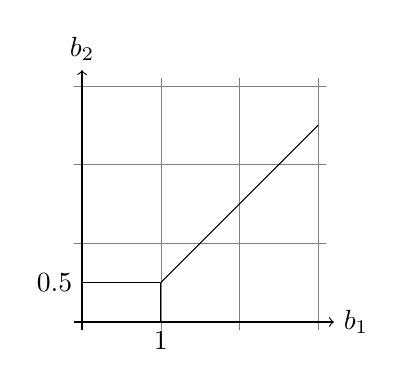
\begin{tikzpicture}
    \draw[very thin,color=gray] (-0.1,-0.1) grid (3.1,3.1);
    \draw[->] (-0.1,0) -- (3.2,0) node[right] {$b_1$};
    \draw[->] (0,-0.1) -- (0,3.2) node[above] {$b_2$};
    \draw[color=black] (1,0)--(1,0.5) ;
    \draw[color=black] (0,0.5)--(1,0.5) ;
    \draw[color=black] (1,0.5)--(3,2.5) ;
    \node[below] at (1,0) {$1$};
    \node[left] at (0,0.5) {$0.5$};
\end{tikzpicture}}
\hfill
\subfigure[Аукцион второй цены]{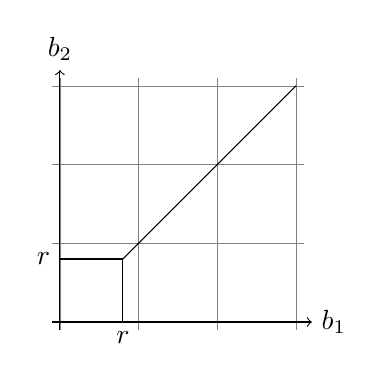
\begin{tikzpicture}
    \draw[very thin,color=gray] (-0.1,-0.1) grid (3.1,3.1);
    \draw[->] (-0.1,0) -- (3.2,0) node[right] {$b_1$};
    \draw[->] (0,-0.1) -- (0,3.2) node[above] {$b_2$};
    \draw[color=black] (0.8,0)--(0.8,0.8) ;
    \draw[color=black] (0,0.8)--(0.8,0.8) ;
    \draw[color=black] (0.8,0.8)--(3,3) ;
    \node[below] at (0.8,0) {$r$};
    \node[left] at (0,0.8) {$r$};
\end{tikzpicture}}
\hfill
\end{figure}

\item Оплата доставки товара покупателем равносильна плате за участие.\index{аукцион!с оплатой доставки} Смотрим задачи из лекции 3. Если покупатель оплачивает доставку сам. То для него — это как плата за участие, но продавец её не получает. Поэтому равновесные стратегии для покупателей, такие же как в аукционе с платой за вход $ w=0.1 $. Величина $ w $ продавцу не достаётся, поэтому его ожидаемый доход уменьшается на $ w(1-\rho) $ и равен:
\begin{equation}
\E(R)=n(n-1)\left(\frac{1}{n(n+1)}-\frac{\rho^{n}}{n}+\frac{\rho^{n+1}}{n+1}\right),\quad \rho=w^{1/n}
\end{equation}


Если же продавец оплачивает доставку сам. То с точки зрения покупателей — это обычный аукцион. А доход продавца надо уменьшить на $ 0.1 $,
\begin{equation}
\frac{n-1}{n+1}-0.1
\end{equation}

Если нарисовать эти функции, то при $ n\geq 3 $ получается, что продавцу выгоднее обещать бесплатную доставку!

\item Механизм VCG: ход делают только жители. Пусть $ X\in[80;180]$ — ход жителей. Принимается решение не строить дорогу, если $ X<90 $, и строить дорогу с помощью двух фирм Б1 и Б2, если $ X\geq 90 $.

Администрация платит 90, если дорога строится и $ X $ если дорога не строится.

Фирма Б1 платит 0, если дорога строится, и $ X-30 $, если дорога не строится.

Фирма Б2 платит 0, если дорога строится, и $ X-60 $, если дорога не строится.

Жители получают 90, если дорога строится, и 0, если дорога не строится.

Баланс всегда неотрицательный.


\item На отрезке $ [0;1] $ синус является монотонно возрастающим. Без применения синуса стратегия «Говорить правду» нестрого доминировала остальные, то есть давала больше денег. С применением синуса стратегия «Говорить правду» дает больший синус количества денег. Но это одно и то же. Значит, стратегия «Говорить правду» по-прежнему нестрого доминирует остальные.

Можно составить табличку для сравнения ходов $ b=x $ и $ b=x-\Delta $.


\end{enumerate}
